\documentclass[preview]{standalone}
\usepackage[table]{xcolor} %load before pgfplots or tikz
\usepackage{pgfplots}
\usepackage{tikz}
\usepackage{tkz-euclide}
\usepackage[font=footnotesize,labelfont=bf]{caption} %change caption size
\pgfplotsset{compat=newest}
\usepgfplotslibrary{fillbetween}

\usetikzlibrary{patterns,angles,calc,quotes,math,intersections,through,positioning,fit,trees,matrix,shadings,shadows}
\usetikzlibrary {arrows.meta,patterns.meta,decorations.pathreplacing,perspective,3d}
\pgfplotsset{compat=newest}

\pgfdeclareverticalshading{groundshading}{2cm}{
	color(0mm)=(white); 
	color(1.9cm)=(black); 
	color(2cm)=(black)
}
\definecolor{cranebody}{HTML}{FFC107}
\definecolor{chainwheel}{HTML}{607D8B}
\definecolor{bodyoutline}{HTML}{37474F}
\definecolor{cranethroat}{HTML}{FB8C00}
\definecolor{throatoutline}{HTML}{AE6100}
\definecolor{cranemirror}{HTML}{BBDEFB}

\begin{document}
    \begin{figure}
        \centering
        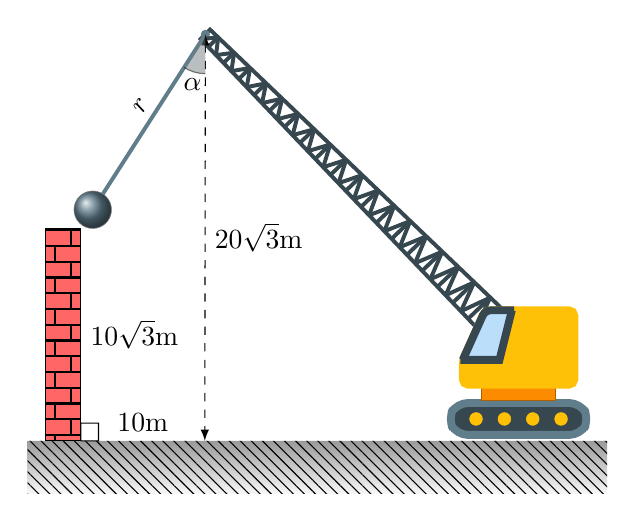
\begin{tikzpicture}[
            scale = 0.75,
            cranewheel/.style = {rounded corners = 4px,line width = 1mm, draw = chainwheel, fill=bodyoutline},
            axle/.style = {draw=cranebody,fill=cranebody},
            throat/.style =  = {fill = cranethroat,draw = throatoutline},
            cranebox/.style = {rounded corners = 2px,line width = 1mm, draw = cranebody, fill=cranebody},
            mirrorframe/.style = {line width = 1mm,draw = bodyoutline},
            cranearm/.style = {line width = 0.5mm,draw = bodyoutline},
            soil/.style = {pattern={Lines[angle=-45,distance={4pt/sqrt(2)}]}},
            anglestyle/.style = {angle radius = 5mm, angle eccentricity = 1.02,fill = bodyoutline!70,opacity = 0.5,draw = black},
            ]
            \tikzmath{
                \scale = 0.3;
                \armlength = 25*\scale;
                \armangle = 45;
                \wallheight = 12*\scale;
                \walldist = 7*\scale;
                \wallwidth = 2*\scale;
                \ballangle = 30;
                \balloffset = 0.02*\scale;
                \ballradius = 0.3*\scale;
                \tipw = 0.1*\scale;
                \bottomw = 0.25*\scale;
                \dcrane = 0;
                \dwheel = 7*\scale;
                \dwheelh = 1.8*\scale;
                \dwheelextrude = 0.5*\scale;
                \numaxle = 4; %number of axles in the wheel
                \axleradius = 0.2*\dwheelh;
                \dax = 1/(\numaxle+1);
                \throat = 0.6*\dwheel;
                \throath = 0.7*\scale;
                \boxw = 0.9*\dwheel;
                \boxh = 0.6*\dwheel;
                \boxm = 0.2*\dwheel;
                \boxroof = 0.8*\boxw;
                \topframew = 0.3*\boxroof;
                \bottomframew = 0.35*\boxw;
                \numseg = 20; %segments in the arm
                \darmU = 1/(\numseg);
                \darmD = 1/(\numseg);
                \groundoffset = 1*\scale;
                \grounddepth = 3*\scale;
            }
            
            %wheel
            \coordinate (centercrane) at ([yshift = 1mm]\dcrane,0);
            \draw[cranewheel] (centercrane)
            -- ++ (180:0.5*\dwheel)
            -- ++ (-\dwheelextrude,0.5*\dwheelh) coordinate (wLeft)
            -- ++ (\dwheelextrude,0.5*\dwheelh) coordinate (wTopLeft)
            -- ++ (0:\dwheel)  coordinate (wTopRight)
            -- ++(\dwheelextrude,-0.5*\dwheelh) coordinate (wRight)
            -- ++ (-\dwheelextrude,-0.5*\dwheelh)
            -- cycle;
            \foreach \i in {1,...,\numaxle}{
                \tikzmath{
                    \proportion = \i*\dax;
                }
                \coordinate (axlecenter) at ($(wLeft)!\proportion!(wRight)$);
                \path (axlecenter) -- ++(90:\axleradius) coordinate (axletop);
                \tkzDrawCircle[axle](axlecenter,axletop);
            }
            %throat
            \coordinate (wTopMid) at ([yshift = 0.5mm]$(wTopLeft)!0.5!(wTopRight)$);
            \draw[fill = cranethroat,draw = throatoutline] (wTopMid)
            -- ++ (180:0.5*\throat)
            -- ++ (90:\throath)
            -- ++ (0:0.5*\throat) coordinate (throatMid)
            -- ++ (0:0.5*\throat)
            -- ++ (270:\throath)
            -- cycle;
            
            %arm
            \coordinate (boxcenter) at ([yshift = 0.5mm]throatMid);
            \path (boxcenter) 
            -- ++ (90:0.5*\boxh) coordinate (boxmid)
            -- ++ (180-\armangle:\armlength) coordinate (pivot);
            \tikzmath{
                \armwidthB = 0.5*\bottomw;
                \armwidthT = 0.5*\tipw;
            }
            \coordinate (armBU) at ($(boxmid)!\armwidthB!-90:(pivot)$);
            \coordinate (armBD) at ($(boxmid)!\armwidthB!90:(pivot)$);
            \coordinate (armTU) at ($(pivot)!\armwidthT!90:(boxmid)$);
            \coordinate (armTD) at ($(pivot)!\armwidthT!-90:(boxmid)$);
            \draw[cranearm] (armTU) -- (armBU) -- (armBD) -- (armTD) -- cycle;
            \tkzDrawPoint[chainwheel,size = 1mm](pivot);
            \foreach \i in {1,...,\numseg}{
                \tikzmath{
                    int \cc;
                    \cc = 1*\i;
                    \propD = (\cc-1)*\darmD;
                    \propDn = (\cc)*\darmD;
                    \propU = (\cc-0.5)*\darmU;
                }
                \coordinate (segup) at ($(armBU)!\propU!(armTU)$);
                \coordinate (segdown) at ($(armBD)!\propD!(armTD)$);
                \coordinate (segdownnext) at ($(armBD)!\propDn!(armTD)$);
                \tkzDefPointBy[projection = onto segdown--segdownnext](segup)\tkzGetPoint{segmid};
                \draw[cranearm,rounded corners = 1px] (segdown) -- (segup) -- (segdownnext);
                \draw[cranearm] (segup) -- (segmid);
            }
            
            %box
            \path (boxcenter) -- ++ (180:0.5*\boxw) -- ++ (90:\boxm) coordinate (boxcorner);
            \draw[cranebox] (boxcenter)
            -- ++ (0:0.5*\boxw)
            -- ++ (90:\boxh)
            -- ++ (180:\boxroof) coordinate (roofbend)
            -- (boxcorner)
            -- ++ (270:\boxm)
            -- cycle;
            
            %mirrorframe
            \path (roofbend) -- ++(0:\topframew) coordinate (topFrameEnd);
            \draw[fill = cranemirror] (boxcorner) -- ++(0:\bottomframew) -- (topFrameEnd) -- (roofbend) -- (boxcorner);
            \draw[mirrorframe] ([xshift=-0.4mm]boxcorner) -- ++(0:\bottomframew) -- (topFrameEnd);
            \draw[mirrorframe,rounded corners = 2px] ([xshift=0.4mm]topFrameEnd) -- (roofbend) -- (boxcorner);
            
            %wall
            \tkzDefPoints{0/0/O,1/0/Ox}
            \coordinate (px) at ([yshift = 1mm]pivot);
            \tkzInterLL(O,Ox)(pivot,px)\tkzGetPoint{pivotbottom}
            
            \path (pivotbottom) -- ++(180:\walldist) coordinate (wallstart);
            \draw[preaction ={fill,red!60}, pattern = bricks] (wallstart)
            -- ++(90:\wallheight) coordinate (wallupperright)
            -- ++(180:\wallwidth)
            -- ++(270:\wallheight) coordinate (wallback)
            -- cycle;
            
            %ball
            \coordinate (balloffset) at ($(wallupperright)!\balloffset!(pivot)$);
            \coordinate (ballcenter) at ($(balloffset)!\ballradius!(pivot)$);
            \coordinate (balltop) at ($(ballcenter)!\ballradius!(pivot)$);
            \draw[chainwheel,line width=0.5mm] (balltop) -- (pivot);
            \tkzDrawCircle[ball color = chainwheel](ballcenter,balltop);
            
            %ground
            \path (wallback)
            -- ++(180:\groundoffset) coordinate (groundstart)
            -- ++ (270:\grounddepth) coordinate (groundbelowstart);
            \path ([yshift = -1mm]wRight) 
            -- ++(270:0.5*\dwheelh)
            -- ++(0:\groundoffset) coordinate (groundend)
            -- ++(270:\grounddepth) coordinate (groundbelowend);
            
            \path[shading = groundshading,opacity = 0.4] (groundstart) -- (groundend) -- (groundbelowend) -- (groundbelowstart) -- cycle;
            \path[soil] (groundstart) -- (groundend) -- (groundbelowend) -- (groundbelowstart) -- cycle;
            
            %annotations
            \draw[dashed,latex-latex] (pivot) -- (pivotbottom) node[midway,right] {$20\sqrt{3}$m};
            \path (wallstart) -- (wallupperright) node[midway,right] {$10\sqrt{3}$m};
            \path (wallstart) -- (pivotbottom) node[midway,above] {$10$m};
            \tkzMarkRightAngle[draw=black,size=1*\scale](pivotbottom,wallstart,wallupperright);
            \pic[anglestyle] {angle=wallupperright--pivot--pivotbottom};
            \tkzDefLine[bisector,normed](wallupperright,pivot,pivotbottom)\tkzGetPoint{angleloc};
            \node[anchor = 80] at ($(pivot)!6mm!(angleloc)$) {$\alpha$};
            \path (balltop) -- (pivot) node[midway,above,sloped] {$r$};
        \end{tikzpicture}
        \caption{Crane with a wrecking ball.}
    \end{figure}
\end{document}
